\documentclass[dvipsnames, svgnames, x11names,border=3pt]{standalone}
\usepackage{tikz,pgfplots}
\usepgfplotslibrary{fillbetween}
\pgfplotsset{compat = 1.18,width=10cm, height=10cm}

\begin{document}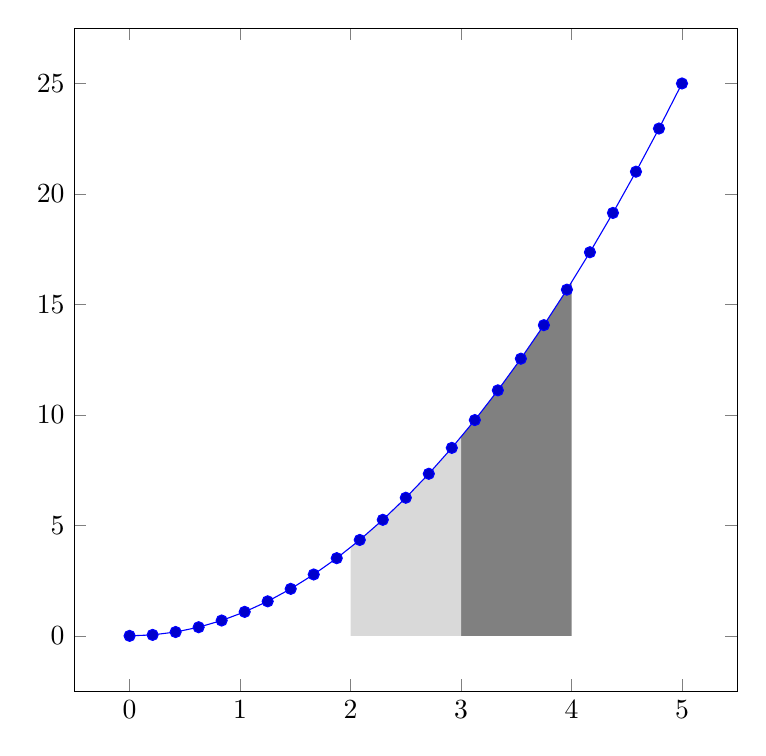
\begin{tikzpicture}\begin{axis}

\addplot+ [name path=A,domain=0:5] {x^2};

\path [name path=B](\pgfkeysvalueof{/pgfplots/xmin},0) --(\pgfkeysvalueof{/pgfplots/xmax},0);

\addplot [gray] fill between [of=A and B,soft clip={domain=3:4}];
\addplot [gray!30] fill between [of=A and B,soft clip={domain=2:3}];


\end{axis}\end{tikzpicture}\end{document}
